%-Document Type------------------------------------------------------------------------------
\documentclass[12pt,a4paper]{report}
%--------------------------------------------------------------------------------------------

%Packages------------------------------------------------------------------------------------
\usepackage[colorlinks=true,linkcolor=blue]{hyperref} %Using this package will automatically turn references into links.
\usepackage{graphicx}
\usepackage{listings} % Required for insertion of code
\usepackage[linesnumbered]{algorithm2e}
\usepackage{tikz}
\usepackage{verbatim}
\usepackage{subcaption}
\usetikzlibrary{trees}
%---------------------------------------------------------------------------------------------

%Preamble-------------------------------------------------------------------------------------

%End Preamble---------------------------------------------------------------------------------

%Document----------------------------------------------------------------------------------------
\begin{document}
\parindent0pt

%Cover Page---------------------------------------------------------------------------------------
\title{COMS3008: Parallel Computing Assignment}
\author{Tau Merand 908096 \and Vincent Varkevisser 705668}
\maketitle
%Cover Page End-----------------------------------------------------------------------------------
\section*{Introduction}
The game of peg solitaire is a one player game played on a 33 holed cross shaped board that involves jumping pegs over other pegs, in a manner similar to checkers. The rules are as follows:
\begin{enumerate}
  \item A move consists of jumping a peg over an orthogonal neighbor into an empty space. The peg that was jumped over is then removed from the board.
  \item Pegs can only jump onto an empty space.
  \item The game is won if the final peg is in the centre space.
  \item If no pegs can legally move or the final peg is not in the centre the game is lost.
\end{enumerate}
\begin{figure}[ht]
  \begin{subfigure}[t]{0.3\textwidth}
    \centering
    \resizebox{\textwidth}{!}{
      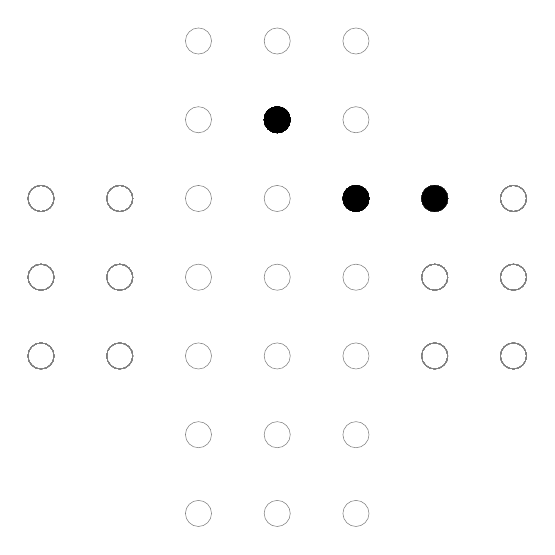
\begin{tikzpicture}
        [empty/.style={circle,draw=gray,very thin}, full/.style={circle,draw=black, fill=black ,very thin}]
        \foreach \x in {2,3,4}
          \foreach \y in {0,1, 2,3,4,5,6}
            \path node at (\x,\y) [empty] {}
                  node at (0,2) [empty] {}
                  node at (0,3) [empty] {}
                  node at (0,4) [empty] {}
                  node at (1,2) [empty] {}
                  node at (1,3) [empty] {}
                  node at (1,4) [empty] {}
                  node at (5,2) [empty] {}
                  node at (5,3) [empty] {}
                  node at (5,4) [empty] {}
                  node at (6,2) [empty] {}
                  node at (6,3) [empty] {}
                  node at (6,4) [empty] {}
                  node at (4,4) [full] {}
                  node at (5,4) [full] {}
                  node at (3,5) [full] {};
      \end{tikzpicture}
    }
    \caption{A start state}
  \end{subfigure}\hfill%
  \begin{subfigure}[t]{0.3\textwidth}
    \centering
    \resizebox{\textwidth}{!}{
      \begin{tikzpicture}
        [empty/.style={circle,draw=gray,very thin}, full/.style={circle,draw=black, fill=black ,very thin}]
        \foreach \x in {2,3,4}
          \foreach \y in {0,1, 2,3,4,5,6}
            \path node at (\x,\y) [empty] {}
                  node at (0,2) [empty] {}
                  node at (0,3) [empty] {}
                  node at (0,4) [empty] {}
                  node at (1,2) [empty] {}
                  node at (1,3) [empty] {}
                  node at (1,4) [empty] {}
                  node at (5,2) [empty] {}
                  node at (5,3) [empty] {}
                  node at (5,4) [empty] {}
                  node at (6,2) [empty] {}
                  node at (6,3) [empty] {}
                  node at (6,4) [empty] {}
                  node at (3,4) [full] {}
                  node at (3,5) [full] {};
      \end{tikzpicture}
    }
    \caption{The right most peg jumps over its left neighbour}
  \end{subfigure}\hfill%
  \begin{subfigure}[t]{0.3\textwidth}
    \centering
    \resizebox{\textwidth}{!}{
      \begin{tikzpicture}
        [empty/.style={circle,draw=gray,very thin}, full/.style={circle,draw=black, fill=black ,very thin}]
        \foreach \x in {2,3,4}
          \foreach \y in {0,1, 2,3,4,5,6}
            \path node at (\x,\y) [empty] {}
                  node at (0,2) [empty] {}
                  node at (0,3) [empty] {}
                  node at (0,4) [empty] {}
                  node at (1,2) [empty] {}
                  node at (1,3) [empty] {}
                  node at (1,4) [empty] {}
                  node at (5,2) [empty] {}
                  node at (5,3) [empty] {}
                  node at (5,4) [empty] {}
                  node at (6,2) [empty] {}
                  node at (6,3) [empty] {}
                  node at (6,4) [empty] {}
                  node at (3,3) [full] {};
      \end{tikzpicture}
    }
    \caption{The winning state}
  \end{subfigure}
  \caption{A winning set of valid moves}
\end{figure}
\pagebreak
\section*{Backtracking Search}
Recursive backtracking using depth first search was chosen as the method for state space exploration. The standard backtracking depth first algorithm is as follows:

\begin{algorithm}[H]
	\DontPrintSemicolon
	\SetKwInOut{Input}{input}
	\SetKwInOut{Output}{output}
	\SetKwData{Result}{result}
	\SetKwData{State}{state}
	\SetKwData{Initial}{initialState}
	\SetKwData{Legal}{legalMoves}
	\SetKwData{Move}{move}
	\SetKwData{Child}{childResult}
	\SetKw{Break}{break}
	\SetKw{Continue}{continue}
	\SetKwFunction{Backtrack}{backtrack}
	\SetKwProg{Fn}{Function}{}{}
	\Fn{\Backtrack}{
		\Input{An initial, possibly un-winnable, board state.} %We can't restrict ourselves to valid states, or we wouldn't be able to recurse.
		\Output{A sequence of moves to get from the initial state to the winning state, if a winning state
			cannot be reached the sequence should be empty.}
		\BlankLine
		\Initial$\leftarrow$ The initial state\;
		\Legal$\leftarrow$ A list of all the legal moves for \Initial\;
		\Result$\leftarrow$ Empty list to store moves from the initial state to the winning state\;
		\ForEach{\Move in \Legal}{
			\State$\leftarrow$ The state after playing \Move on \Initial\;
			\If{\State is a winning state}{
				\Result$\leftarrow$ \Move\;
				\Break\;
			}
			\BlankLine
			\Child$\leftarrow$ \Backtrack{\State}\;
			\BlankLine
			\If{\Child is not empty}{
				Prepend \Move to \Child\;
				\Result$\leftarrow$ \Child\;
				\Break\;
			}
		}
		\BlankLine
		\Return{\Result}\;
	}
	\caption{A standard recursive backtracking using DFS}
\end{algorithm}

But because pegs are indistinguishable, game states where pegs are in the same position are identical, regardless of the moves taken to arrive at that state. Thus exploring the state space looking for a sequence of states leading to the winning state will probably involve evaluating the same states many times. Thus a significant speed up can be achieved by saving states that are known to not lead to the winning state as in the following algorithm:

\begin{algorithm}[H]
	\DontPrintSemicolon
  \label{dyn-alg}
	\SetKwInOut{Input}{input}
	\SetKwInOut{Output}{output}
	\SetKwData{Result}{result}
	\SetKwData{State}{state}
	\SetKwData{Initial}{initialState}
	\SetKwData{Legal}{legalMoves}
	\SetKwData{Move}{move}
	\SetKwData{Child}{childResult}
	\SetKwData{Dataset}{infeasibleSet}
	\SetKw{Break}{break}
	\SetKw{Continue}{continue}
	\SetKwFunction{Backtrack}{dynamicBacktrack}
	\SetKwProg{Fn}{Function}{}{}
	\Fn{\Backtrack}{
		\Input{An initial, possibly un-winnable, board state.}
		\Input{A set of all states that have been searched and are known to be un-winnable.}
		\Output{A sequence of moves to get from the initial state to the winning state, if a winning state
			cannot be reached the sequence should be empty.}
		\BlankLine
		\Initial$\leftarrow$ The initial state\;
		\Dataset$\leftarrow$ The set of un-winnable states\;
		\Legal$\leftarrow$ A list of all the legal moves for \Initial\;
		\Result$\leftarrow$ Empty list to store moves from the initial state to the winning state\;
		\ForEach{\Move in \Legal}{ \label{loop}
			\State$\leftarrow$ The state after playing \Move on \Initial\;
			\BlankLine
			\If{\State is in \Dataset}{
				\Continue\;
			}
			\BlankLine
			\If{\State is a winning state}{
				\Result$\leftarrow$ \Move\;
				\Break\;
			}
			\BlankLine
			\Child$\leftarrow$ \Backtrack{\State, \Dataset}\;
			\BlankLine
			\uIf{\Child is not empty}{
				Prepend \Move to \Child\;
				\Result$\leftarrow$ \Child\;
				\Break\;
			}
			\Else{
				Add \State to \Dataset\;
			}
		}
		\BlankLine
		\Return{\Result}\;
	}
	\caption{Recursive backtracking using DFS and dynamic programming methods}
\end{algorithm}

\subsection*{Parallel Implementation}
To parallelise the above algorithms it was decided to make use of the openmp parallel for loop to allow the concurrent depth first exploration of multiple moves from the initial state. The openmp parallel for loop partitions the iteration space of the loop at \autoref{loop} of Algorithm~\autoref{dyn-alg}.

Static, dynamic and guided openmp load balancing constructs were all tried, but dynamic gave by far the best performance. This is because dynamic (with default chunk size) gives one element of the iteration space to a thread at a time, allocating new tasks to threads as they finish their allocated task in a round robin approach. This gives good load balancing in this particular problem since some elements of the iteration space may require exploring the game graph very deeply while others may quickly lead to previously seen infeasible states.

The infeasible set is an instance variable of the object and as such each thread can concurrently reference it. Simultaneously, concurrent threads writing to the infeasible set need to avoid data races. Thus the function to add a state to the infeasible set must be an openmp critical region.

Nested parallelism was also tried and was found to be highly inefficient. Further various upper limits on the depth with which nested parallelism could take place wee tried but the added overhead of parallelism within the recursive algorithm remained slower than no nested parallelism at all.

\pagebreak

\section*{Results}
\graphicspath{ {TestData/} }
\begin{figure}[ht]
  \includegraphics[width=\linewidth]{better_graph2}
  \caption{Graph comparing running times of serial and parallel implementations of Algorithm~\ref{dyn-alg}}
  \label{grph}
\end{figure}
As can be seen in \autoref{grph} the parallel algorithm is generally faster than the serial, but we did not see the $\frac{n}{p}$ kind of performance gains one naively expects from parallelism. This is possibly due to the recursive nature of our implementation and our dynamic programming approach.



\end{document}
